\pagebreak
\section{Training API Pattern Identification}\label{sec:pattern}

\subsection{Training API Patterns of TensorFlow DL Models}

\begin{figure}[ht!]
\centering
  \begin{subfigure}[b]{\textwidth}
    \begin{lstlisting}[style=mpython]
for x, y in train_data.take(training_steps):
    with tf.GradientTape() as tape:
        pred = model(x, is_training=True)
        loss = loss_compute(y, pred)

    trainable_vars = model.trainable_variables
    gradients = tape.gradient(loss, trainable_vars)
    pairs = zip(gradients, trainable_vars)
    optimizer.apply_gradients(pairs)\end{lstlisting}
    \caption{Using low-level training API}
  \end{subfigure}
  \hspace{5mm}
  \begin{subfigure}[b]{\textwidth}
    \begin{lstlisting}[style=mpython]
model.compile(
    optimizer = optimizer, 
    loss = loss_compute) 
model.fit(train_data.take(training_steps))\end{lstlisting} 
    \caption{Using high-level training API}
  \end{subfigure}

  \caption{TensorFlow model code example using two different API patterns}
  \label{fig:pattern:ex01}
\end{figure}

% tf 모델을 바르게 변환하기 위해서는,  서로 다른 훈련 api를 사용하느 ㄴ모델을
% 분류하고, 각 분류의 모델에 다른 변환을 적용할 필요가 있다.
TensorFlow offers multiple APIs for defining the structure of the model and the
training process. 
These APIs include low-level APIs such as {\tt tf.GradientTape} and high-level
APIs such as {\tt tf.keras.Model}.
The choice of API depends on the model' complexity and the project's specific
requirements.
Figure \ref{fig:pattern:ex01} illustrates two TensorFlow model codes that use
different APIs to define the training process. 
Figure~\ref{fig:pattern:ex01}(a) explicitly repeats the training
steps using the {\tt for} loop and the {\tt GradientTape} instance. 
On the other hand, Figure~\ref{fig:pattern:ex01}(b) uses the Keras
library APIs, {\tt compile} and {\tt fit}, to set a training methodology of the
model and invoke the training process. 
While both codes train the model similarly, they use different training
APIs in different patterns.

Our transformation approach needs to apply different transformation rules based
on the API usage in the TensorFlow model. 
Inspecting the Horovod documentation and open-source TensorFlow models
manually, we define four categories of training API patterns that require
different transformation rules. 
The training API patterns are the code patterns of TensorFlow API calls that
commonly appear in the models belonging to the same categories.
For instance, models in the {GradientTape} category commonly use a {\tt with}
statement to create a {\tt GradientTape} object, as illustrated in
Figure~\ref{fig:pattern:ex01}(a).
We define patterns for such common API usages, and our tool identifies the
training API patterns of given models automatically to choose appropriate
transformation rules for the models.

Table~\ref{tab:patterns} represents the four training API patterns. 
The first column shows TensorFlow versions on which models are built, and the
second and third columns show training API pattern names and descriptions,
respectively.
We provide a detailed description of each pattern in the subsequent paragraphs
and then present an algorithm that identifies the categories of models in
Section~\ref{sec:ident}.

%In TensorFlow models, developers can use different APIs to define the 
%model structure and training process.
%The figure \ref{fig:pattern:ex01} illustrates two TensorFlow model codes that
%use different APIs to define the training process.
%The lines 2 to 10 in \ref{fig:pattern:ex01}(a)  
%explicitly repeats the training steps by using the {\tt for} loop
%and the {\tt GradientTape} instance.
%In contrast, the lines 1 and 4 in \ref{fig:pattern:ex01}(b) use the Keras
%library APIs, {\tt compile} and {\tt fit}, to set a training methodology of the
%model and invoke the training process.
%While both codes train the model in the same way, they use different training 
%APIs in different patterns.
%As their API usages are significantly different, our transformation approach
%need to apply different transformation rules.

\begin{table}[ht!]
  \centering
  \caption{Four types of training API patterns}
  \begin{tabular}{|c|c|l|}
    \hline
    TF version & API Pattern & Description \\
    \hline
    1.x & Session & 
	  Using the {\tt Session} API to invoke training operations\\
    \hline
    1.x & MonitoredSession & 
      Using the {\tt MonitoresSession} API to invoke training operations.\\
    \hline
    2.x & GradientTape & 
      Using the {\tt GradientTape} API to explicitly repeat the training
      step.\\
    \hline
    2.x & Keras & 
      Using the {\tt keras.Model} class to define the model and the {\tt fit} API
      to train the model.\\
    \hline
  \end{tabular}
  \label{tab:patterns}
\end{table}

% 서로 다은 훈련 api를 사용하는 모델을 분류하기 위해서 우리는 4개의
% training api pattern을 정의햇다.
%To categorize the TensorFlow DL models by their training API usage,
%we manually inspected open-source TensorFlow models and
%defined four \textit{training API patterns} that categorizes them.
%The training API patterns are the code patterns of TensorFlow APIs 
%that commonly appear in the same categories of the models.
%For instance, the models in the same category with the figure
%\ref{fig:pattern:ex01}(a) use the {\tt with} statements that create the
%{\tt GradientTape} objects.
%We patternize such common API usages into the training API patterns and
%utilize to categorize the TensorFlow DL models.
%Figure \ref{tab:patterns} describe the four training API patterns defined
%for TensorFlow DL models.
%The following paragraphs explain the details of each training API pattern.



% 우리가 정의한 4가지의 api pattern은 피규어의 표와 같다. 
% Figure \ref{tab:patterns} describes the four training API patterns.
% The Session pattern and the MonitoredSession pattern categorizes the
% TensorFlow 1.x models. The GradientTape pattern and the Keras pattern
% categorizes the TensorFlow 2.x models.
% Based on the training API patterns,
% we implement the \textit{training API pattern identifier} to
% categorize the input model.
% The training API pattern identifier matches each training API pattern
% against the input model codes. 
% If the code successfully matches in exactly one pattern,
% the training API pattern identifier categorizes the input model into
% the corresponding pattern.
% If the code fails to match a pattern or is matched into more than one patterns,
% the training API pattern identifier raises exception that the input model
% cannot be automatically transformed by our approach.


\paragraph{Session Pattern.} 
The Session pattern appears in TensorFlow 1.x models that invoke the training
computation directly via the {\tt Session} class instance.
Figure~\ref{fig:sessionpattern} illustrates a code example of the Session
pattern. 
The {\tt with} statement in line 1 creates an instance of the {\tt Session}
class, and the {\tt run} method called in line 3 invokes the training
computation on an isolated execution environment of the session instance. 
The {\tt run} method is usually called multiple times through a loop statement
to train models on several training batches.
\vspace{-1em} 

\begin{figure}[!ht]
\begin{lstlisting}[style=mpython]
with tf.Session() as sess:
    for images, labels in dataset.take(10000):
        sess.run(train_op, {x: images, y: labels})
\end{lstlisting}
\caption{Session pattern code example}
\label{fig:sessionpattern}
\end{figure}
\vspace{-1em} 


%To identify the Session pattern model, the identifier 
%searches for a {\tt with} statement that creates the {\tt Session} instance.
%If the body statements of the {\tt with} statement call the 
%{\tt run} method of the {\tt Session} instance,
%the identifier categorizes the input model as the Session pattern. 


\paragraph{MonitoredSession Pattern.}
The MonitoredSession is another typical code pattern observed in
TensorFlow 1.x models. 
Figure~\ref{fig:monsesspattern} demonstrates a code example of the
MonitoredSession pattern.
This pattern bears similarities to the Session pattern, wherein the training
computation is invoked directly.
However, instead of utilizing an instance of the {\tt Session} class, the
MonitoredSession pattern leverages an instance of the {\tt
MonitoredSession} class that provides hooks to perform some actions
automatically on specific conditions during the training.
The {\tt with} statement in line 3 creates an instance of the {\tt
MonitoredSession} class via the {\tt MonitoredTrainingSession} API, and the
{\tt run} method call in line 5 invokes the training computation.
The {\tt SummarySaverHook} API call in line 1 creates one of the pre-defined
hooks, which saves the model summaries after each training step. 
TensorFlow provides the {\tt TensorBoard} utility visualizing model summaries,
so that model engineers can check training processes from the summaries.
\vspace{-1em} 

\begin{figure}[!ht]
  \begin{lstlisting}[style=mpython]
summary_hook = SummarySaverHook(...)

with MonitoredTrainingSession(hooks=[summary_hook]) as mon_sess:
    while not mon_sess.should_stop():
        mon_sess.run(train_op, feed_dict=feed_dict)\end{lstlisting}
  \caption{MonitoredSession pattern code example}
  \label{fig:monsesspattern}
\end{figure}

%To identify the MonitoredSession pattern training code,
%the identifier searches for a {\tt with} statement that creates a
%{\tt MonitoredSession} instance by {\tt MonitoredTrainingSession} API.
%If the body statements of the {\tt with} statement call the {\tt run} methods 
%of the {\tt MonitoredSession} instance, 
%the identifier categorizes the input model as the MonitoredSession pattern. 
\vspace{-1em} 

\paragraph{GradientTape Pattern.}
The GradientTape pattern is a classification for TensorFlow 2.x models that
utilize the {\tt GradientTape} class instance to initiate training computations
manually.
Figure~\ref{fig:tapepattern} demonstrates an example of the
GradientTape pattern. 
Line 4 initiates the {\tt GradientTape} class instance through a {\tt with}
statement. 
Once creating the {\tt GradientTape} instance, it watches all trainable
variables by default and records operations executed on the variables within
its context manager.
The {\tt gradient} method call in line 7 calculates and returns gradients from
the recorded operations and the watched variables. 
Finally, in line 9, the {\tt apply\_gradients} method of the {\tt Optimizer}
class instance is called to update the model parameters.

%The GradientTape pattern categorizes TensorFlow 2.x models that
%use the {\tt GradientTape} class instance to manually invoke training 
%computations. Figure \ref{fig:tapepattern} is a code example of 
%GradientTape pattern.
%In line 3, the {\tt with} statement creates the {\tt GradientTape} class
%instance. 
%After the {\tt with} statement, the line 8 calls the {\tt gradient} method
%to retreive the recorded gradients of the model.
%The line 9 calls the {\tt apply\_gradients} methods of the {\tt Optimizer}
%class instance to finally update the model parameters.
\vspace{-1em} 

\begin{figure}[!ht]
  \begin{lstlisting}[style=mpython]
optim = tf.optimizers.Adam(0.001)

for images, labels in dataset.take(10000):
    with tf.GradientTape() as tape:
        probs = model(images)
        loss_value = loss(labels, probs)
    grads = tape.gradient(loss_value, model.trainable_variables)
    optim.apply_gradients(zip(grads, model.trainable_variables))\end{lstlisting}
  \caption{GradientTape pattern code example}
  \label{fig:tapepattern}
\end{figure}

%The GradientTape pattern categorizes TensorFlow 2.x models that
%use the {\tt GradientTape} class instance to manually invoke training 
%computations. Figure \ref{fig:tapepattern} is a code example of 
%GradientTape pattern.
%In line 3, the {\tt with} statement creates the {\tt GradientTape} class
%instance. 
%After the {\tt with} statement, the line 8 calls the {\tt gradient} method
%to retreive the recorded gradients of the model.
%The line 9 calls the {\tt apply\_gradients} methods of the {\tt Optimizer}
%class instance to finally update the model parameters.

%To identify a GradientTape pattern model,
%the identifier searches for the {\tt with} statement that creates a
%{\tt GradientTape} instance.
%The identifier also searches for the {\tt Optimizer} instance 
%{\tt apply\_gradients} method call.
%If identifier finds both of the statements, the identifer categorizes the
%model as the GradientTape pattern.


\paragraph{Keras Pattern.}
The Keras pattern is another classification for TensorFlow 2.x models that
utilize the keras library in both model creations and training. 
Figure~\ref{fig:keraspattern} represents an example of the Keras pattern.
Line 1 defines the {\tt ResNet} class inherited from the {\tt keras.Model}
class. 
As described in Section~\ref{sec:cha}, the {\tt keras.Model} class provides a
convenient way to construct and train models. 
Line 5 constructs a model as an instance of the {\tt ResNet} class.
Finally, the {\tt fit} method invoked in line 6 trains the model with the given
dataset.

%The Keras pattern categorizes TensorFlow 2.x models that use
%the {\tt keras.Model} class method {\tt fit} to train the model. 
%Figure \ref{fig:keraspattern} is a code example of Keras pattern.
%The line 1 defines the {\tt ResNet} class that inherits the 
%{\tt keras.Model} class. 
%The line 5 creates the {\tt ResNet} class instance.
%The line 6 calls the {\tt fit} method to train the model.
%Note that the {\tt fit} method is inherited from the {\tt keras.Model} class.
\vspace{-1em} 

\begin{figure}[ht!]
  \begin{lstlisting}[style=mpython]
class ResNet(keras.Model):
    def __init__(self, params):
        ...

model = ResNet([2, 2, 2], num_classes)
model.fit(dataset, epochs=50)\end{lstlisting}
 
  \caption{Keras pattern code example}
  \label{fig:keraspattern}
\end{figure}
\vspace{-1em} 

%To identify a Keras pattern model, the identifer searches for the
%{\tt Model.fit} method call. The training API pattern identifier utilizes the
%class inheritance information provides by the class hierarchy analyzer to
%recognize subclasses of the {\tt keras.Model} class and their instances.
%If identifier find the {\tt fit} method call of the {\tt keras.Model} subclass
%instance, the identifier categorizes the model as the Keras pattern.

\subsection{Training API Pattern Identifier}\label{sec:ident}
We implemented \tapi, which classifies a TensorFlow model into one of four
training API patterns. 
Our approach traverses the input model AST to identify statements that match
one of these patterns. 
Note that the input model may not contain any statements or may contain
multiple statements that match the training API patterns. 
In such cases, the identifier must inform the user that the input model is
unsuitable for the automatic transformation.

\begin{figure}[ht!]
  \centering
  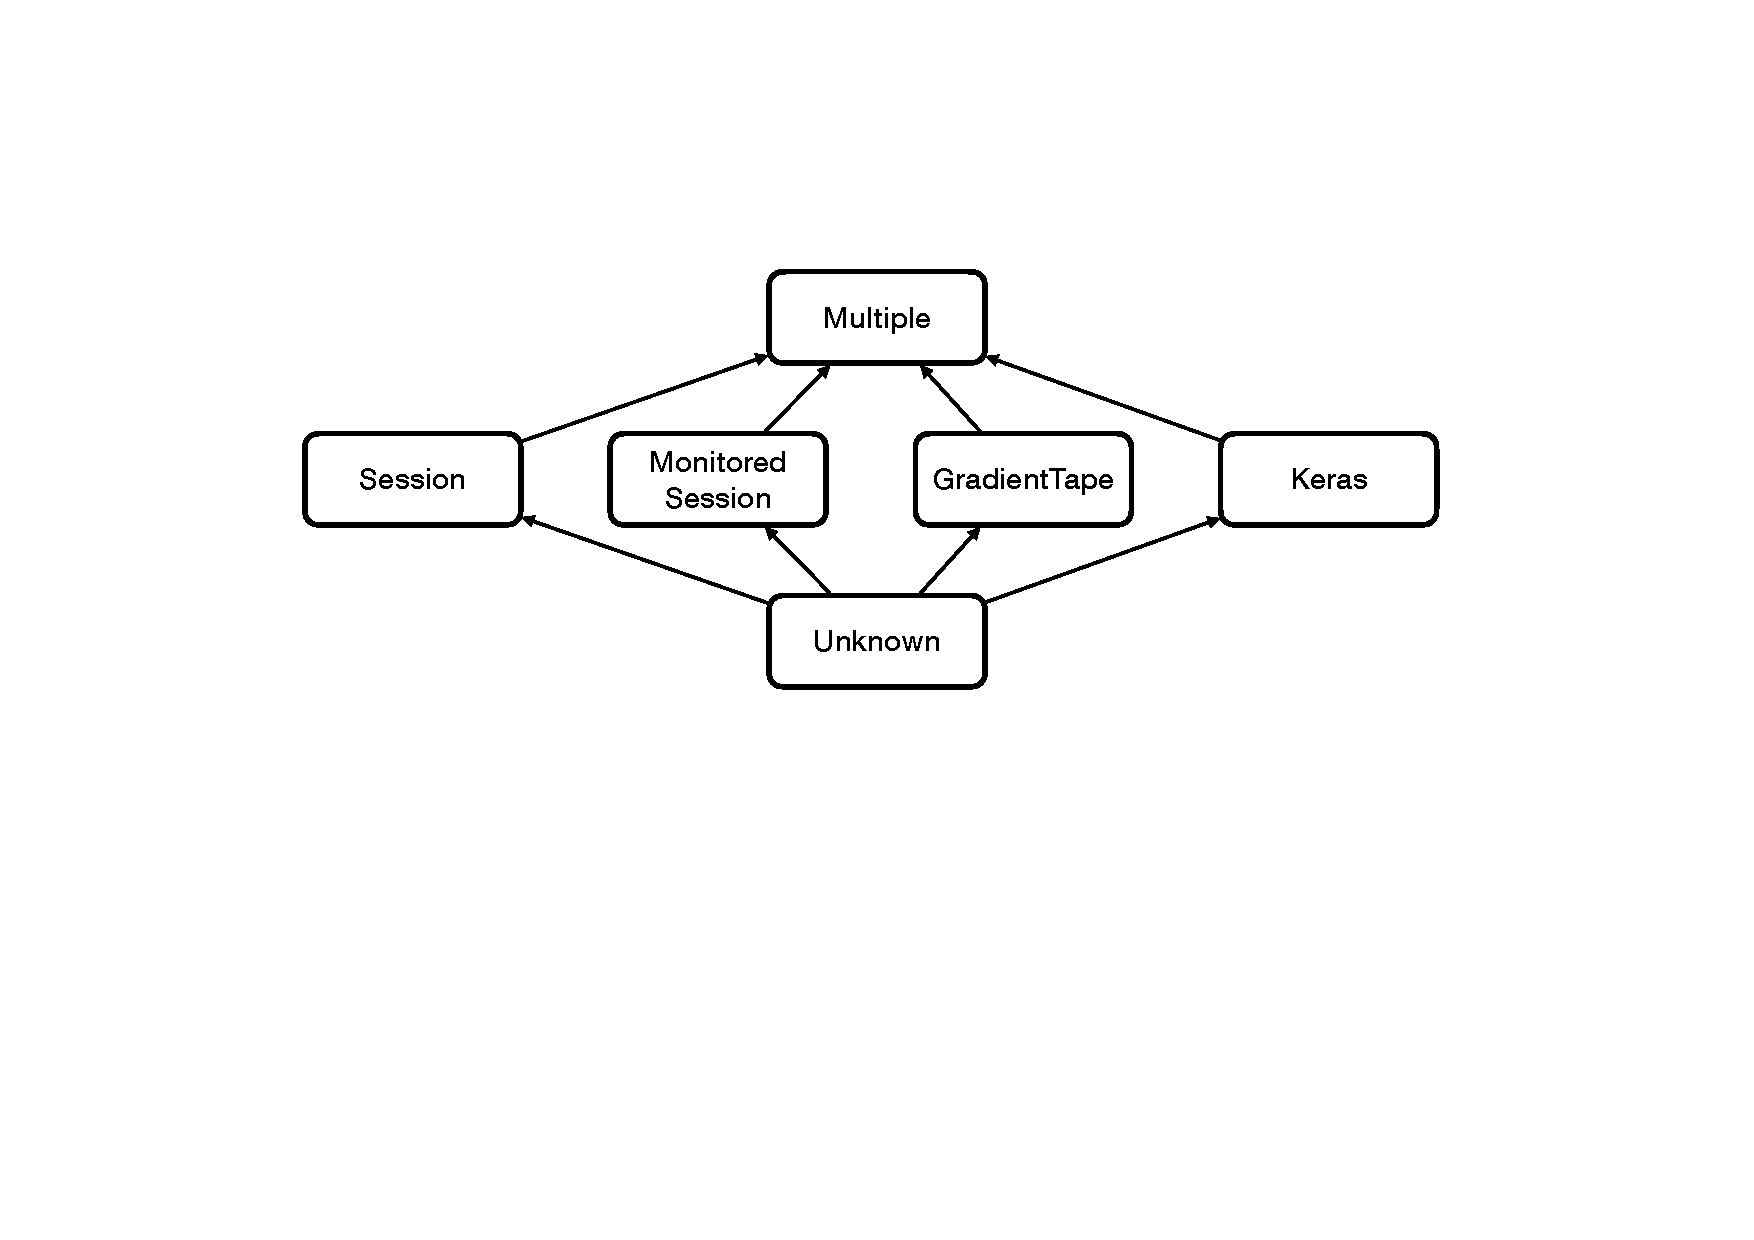
\includegraphics[width=0.6\textwidth]{lattice.pdf}
  \caption{Flat lattice for the training API pattern identification}
  \label{fig:pattern:lattice}
\end{figure}

To handle these scenarios, \tapi~performs a simple static analysis with a flat
lattice domain composed of the four training API patterns, and {\it
Unknown} and {\it Multiple} elements. 
The Unknown element represents that an AST does not match any of the four
training API patterns, and the Multiple element represents that an AST matches
multiple training API patterns.
Figure~\ref{fig:pattern:lattice} depicts the lattice structure.  
The lattice represents a partially ordered set $(P, \sqsubseteq)$ of which the
boxes denote elements in $P$, and the directed edges denote the given order
$\sqsubseteq$ between their {\it from} elements and their {\it to} elements.
The order is a binary relation on the set $P$, which is reflexive ($\forall x
\in P.\ x \sqsubseteq x$), antisymmetric ($\forall x, y \in P.\ x \sqsubseteq y
\wedge x \not= y \to y \not\sqsubseteq x$), and transitive ($\forall x, y, z
\in P.\ x \sqsubseteq y \wedge y \sqsubseteq z \to x \sqsubseteq z$). 
We also define an internal binary operation on the set $P$, denoted as the
symbol $\sqcup$ and named {\it join}, which computes the least upper bound
$lub$ of arbitrary two elements $x$ and $y$ in $P$ as follows: $x \sqsubseteq
lub \wedge y \sqsubseteq lub \wedge \forall ub \in \{e\ |\ x \sqsubseteq e
\wedge y \sqsubseteq e\}.\ lub \sqsubseteq ub$. 
\tapi~applies the join operation to produce one identification result from a
model in which the statements match multiple training API patterns.
For example, the Session element results from joining Session and Unknown
elements, and the Multiple element results from joining MonitoredSession and
Keras elements.

Algorithm~\ref{al:apiident} describes the pseudocode of the training API
pattern identification.
The function {\tt IdentifyPattern} takes both an input AST and the class
hierarchy analysis result, traverses the AST to identify its training API
pattern, and returns it.
The algorithm first tries to match the AST with four training API patterns.
The case statement in
lines~\ref{alg:begin-match-session}~and~\ref{alg:end-match-session}~checks
whether the AST is a {\tt with} statement that creates a {\tt Session} instance
and calls the {\tt run} method of the instance in the body statements.  If the
match succeeds, the algorithm returns the Session element as the AST's
identified training API pattern.
The case statement in
lines~\ref{alg:begin-match-monitoredsession}~and~\ref{alg:end-match-monitoredsession}~checks
whether the AST is a {\tt with} statement that creates a {\tt MonitoredSession}
instance and calls the {\tt run} method of the instance in the body statements.
If the match succeeds, the algorithm returns the MonitoredSession element.
The case statement in line~\ref{alg:begin-match-gradient} checks whether the
AST is a {\tt with} statement that creates a {\tt GradientTape} instance.
Line~\ref{alg:mid-match-gradient} also checks whether the parent AST has a
child statement that calls the {\tt apply\_gradients} method of the instance.
If both matches succeed, the algorithm returns the GradientTape element.
The case statement in line~\ref{alg:begin-match-keras} checks whether the AST
is a {\tt call} statement that invokes the {\tt fit} method of the object
assigned into an arbitrary variable $model$.
The algorithm then analyzes the object's class type by tracking the variable's 
definition site and tests whether the class is a subclass of
the {\tt keras.Model} using the class hierarchy analysis result.
If the match succeeds, the algorithm returns the Keras element.
Lines~\ref{alg:begin-ow}~to~\ref{alg:end-ow}~operate when the input AST
does not match with any of the four training API patterns.
The code invokes the {\tt IdentifyPattern} function recursively for each child
of the AST, joins all the results of the function calls, and returns the join
operation result as the training API pattern.
If the AST has no children, the algorithm identifies it as Unknown.

\atran~transforms an input model via appropriate transformation rules,
depending on the model's training API pattern identified by \tapi.
When the identified pattern is Multiple or Unknown, our tool fails
to transform the model automatically and terminates. 
Note that the transformation failures are rare because our evaluation shows
that \tapi~identifies only one of the 16 target TensorFlow models as Multiple
or Unknown.

%\tapi~finally identifies the input model as one of the six elements.
%If the identified pattern is either Multiple or Unknown, our tool fails to
%transform the model in the automated way and terminates. 
%Otherwise, \atran~transforms the model via appropriate transformation rules,
%depending on the identified pattern.
%Note that the transformation failures are rare in that our evaluation shows
%that the tool identifies only one of the 16 target TensorFlow models as either
%Multiple or Unknown.


%When traversing an input TensorFlow model AST, \tapi~identifies a training API
%pattern for each statement and produces one of the six elements of the lattice.
%The {\it unknown} element, on the third level, indicates that the statement
%does not match match any of the training API patterns. 
%The four elements, on the second level, indicate that the statement matches
%exactly the one corresponding training API patterns.
%The {\it multiple} element, on the first level, indicates that the statement
%matches multiple training API patterns. 
%contains statements that match more than one of the training API patterns. 
%In either case, the input model is deemed unsuitable for automatic
%transformation, resulting in the termination of the transformation process.

%We implemented the training API pattern identifier, which classifies the
%input TensorFlow model into one of the four patterns.
%The training API pattern identifier scans through the input model AST,
%detects statements that match one of the four traning API patterns.
%One caveat here is that the input model can no statements or multiple statements
%that match the training API patterns.
%In these cases, the identifier must notify user that the
%input model is not available for automatic transformation.
%To implement this, we define a flat lattice structure composed of four 
%training API patterns and the top and bottom elements.
%The lattice structure is described in figure \ref{fig:pattern:lattice}.
%The training api pattern identifier returns one of the six elements of
%the lattice. The bottom element means that the input model does not have
%statements that matches with the training API patterns.
%The top elements means that the input model has statements that matches with
%more than one of the training API patterns.
%In both cases, the input model is not available for the automatic 
%transformation, resulting in abortion of the tranformation process.


% TODO put algorithm blocks inside the figure env.
% algo related macro
\algblockdefx{Match}{EndMatch}{\textbf{Match}}{}
\algblockdefx{Case}{EndCase}{\textbf{case}}{}
\algtext*{EndMatch}
\algtext*{EndCase}

\algblockdefx{Enum}{EndEnum}{\textbf{Enum}}{}
\algtext*{EndEnum}

% lattice
% \begin{algorithm}[ht!]
%   \caption{Training API pattern lattice}
%   \begin{algorithmic}[1]
%     \Enum~Pattern
%     \State Top
%     \State SessionPattern 
%     \State MonitoredSessionPattern
%     \State GradientTapePattern
%     \State KerasPattern
%     \State Bot
%     \EndEnum
%     
%     \Function{Union}{$x$, $y$} \Comment{Union of two Patterns, x $\cup$ y}
%     \Match~($x$, $y$)~\textbf{with:}
%       \Case~(Bot, $p$) | ($p$, Bot): $p$ \EndCase
%       \Case~\_: Top \EndCase
% 
%     \EndMatch 
%     \EndFunction
%   \end{algorithmic}
%   \label{fig:pattern:algo1}
% \end{algorithm}

% pseudocode

%\begin{algorithm}
%  \caption{Training API pattern identifier}\label{al:apiident}
%  \begin{algorithmic}[1]
%    \Function{IdentifyPattern}{$AST$}
%    \Match~$AST$~\textbf{with:}
%
%      \Case~{\tt with Session() as}~$name$~{\tt :}~$body$
%        \If{$body$~includes~$name${\tt.run()}}
%          SessionPattern
%        \EndIf
%      \EndCase
%
%      \Case~{\tt with MonitoredTrainingSession() as}~$name$~{\tt :}~$body$
%        \If{$body$~includes~$name${\tt.run()}}
%          MonitoredSessionPattern
%        \EndIf
%      \EndCase
%
%      \Case~{\tt with GradientTape() as}~$name$~{\tt :}~$body$
%        \If{$AST$.parent~includes~$name${\tt.apply\_gradients()}}
%          GradientTapePattern
%        \EndIf
%      \EndCase
%
%      \Case~$model${\tt.fit(...)}
%        \If{$model$.class~isSubclassOf~{\tt keras.Model}}
%          KerasPattern
%        \EndIf
%      \EndCase
%
%      \Case~\_
%        \If{$AST$.isSimpleStatement}
%          Bot 
%        \Else
%          \State \textbf{Let} childrenPatterns \textbf{=} $AST$.childrenStatements.map(s => IdentifyPattern(s))
%          \State childrenPatterns.fold((p1, p2) => p1 $\cup$ p2) 
%        \EndIf
%      \EndCase
%
%    \EndMatch
%    \EndFunction
%  \end{algorithmic}
%\end{algorithm}

\renewcommand{\algorithmicrequire}{\textbf{Input:}}
\renewcommand{\algorithmicensure}{\textbf{Output:}}

\algblockdefx[Foreach]{Foreach}{Endforeach}[2]{\textbf{for each} $#1$ \textbf{in} $#2$}{}
\algblockdefx[Match]{Matchwith}{Endmatch}[1]{\textbf{match} $#1$ \textbf{with}}{}
\algblockdefx[Case]{Matchcase}{Endcase}[1]{\textbf{case} {\tt #1} \textbf{:}}{}
\algblockdefx[Otherwise]{Other}{Endother}{\textbf{otherwise} \textbf{:}}{}
\algtext*{Endforeach}
\algtext*{Endmatch}
\algtext*{Endcase}
\algtext*{Endother}

\begin{algorithm}
  \caption{Training API pattern identification}\label{al:apiident}
  \begin{algorithmic}[1]
    \Require an abstract syntax tree ($ast$) and the class hierarhcy analysis result ($cha$)
    \Ensure the identified training API pattern
    \Function{IdentifyPattern}{$ast$, $cha$}
    \Matchwith{ast}

      \Matchcase{with Session() as $name$ : $body$}\label{alg:begin-match-session}
        \If{$body$~includes~$name${\tt.run()}}
          Session
        \EndIf
      \Endcase\label{alg:end-match-session}

      \Matchcase{with MonitoredTrainingSession() as $name$ : $body$}\label{alg:begin-match-monitoredsession}
        \If{$body$~includes~$name${\tt.run()}}
          MonitoredSession
        \EndIf
      \Endcase\label{alg:end-match-monitoredsession}

      \Matchcase{with GradientTape() as $name$ : $body$}\label{alg:begin-match-gradient}
        \If{$ast$.parent~includes~$name${\tt.apply\_gradients()}}\label{alg:mid-match-gradient}
          GradientTape
        \EndIf
      \EndCase\label{alg:end-match-gradient}

      \Matchcase{$model$.fit(...)}\label{alg:begin-match-keras}
        \If{$cha$.isSubclassOf(type($model$), {\tt keras.Model}))}
          Keras
        \EndIf
      \Endcase\label{alg:end-match-keras}
      \Other
        \State $pattern$ $\leftarrow$ Unknown\label{alg:begin-ow}
        \Foreach{child}{ast\text{.children}}
          \State $pattern$ $\leftarrow$ $pattern$ $\sqcup$ {\sc IdentifyPattern($child$, $cha$)}
        \Endforeach
        \State $pattern$\label{alg:end-ow}
      \Endother
    \Endmatch
    \EndFunction
  \end{algorithmic}
\end{algorithm}

%Algorithm~\ref{al:apiident} describes the pseudocode of the training API
%pattern identifier.
%The function {\tt IdentifyPattern} gets and input AST and returns a training
%API pattern lattice element.
%The algorithm first matches the statement with four training API patterns.
%Lines 3 and 4 match if the input AST is a {\tt with} statement that
%creates a {\tt Session} instance and call the {\tt run} method in the body.
%If the match succeeds, the algorithm returns Session pattern.
%Lines 5 and 6 match if the input AST is a {\tt with} statement that
%creates a {\tt MonitoredSession} instance and call the {\tt run} method in the
%body.
%If the match succeeds, the algorithm returns MonitoredSession pattern.
%Line 7 matches if the input AST is a {\tt with} statement that
%creates a {\tt GradientTape} instance.
%Line 8 then matches if the parent AST has a child statement that calls the
%{\tt apply\_gradients} method of the {\tt GradientTape} instance.
%If both matches succeed, the algorithm returns GradientTape pattern.
%Line 9 and 10 matches if the input AST is a statement that calls
%the {\tt fit} method of a subclass of {\tt keras.Model}. 
%If the match succeeds, the algorithm returns Keras pattern.
%
%Lines 11 to 15 describe the cases where the input AST does not match with 
%one of the four training API patterns.
%If the input AST is a simple statement, which does not have child ASTs,
%the algorithm returns the bottom element.
%Else, the algorithm recursively identifies the pattern of the child ASTs
%then return the join of the results.
%If the child ASTs are matched with multiple training API patterns, 
%the algorithm will return the top element.

